\documentclass[a4paper,openright, 14pt]{article}
\usepackage[utf8]{inputenc}
\usepackage{rotating, graphicx}
\usepackage{tikz}
\usetikzlibrary{datavisualization}
\usetikzlibrary{datavisualization.formats.functions}

\graphicspath{ {./images/} }

\usepackage{fullpage}
\newcommand{\ssection}[1]{%
\section[#1]{\centering\normalfont\scshape #1}}
\newcommand{\ssubsection}[1]{%
\subsection[#1]{\bfseries\normalfont\scshape #1}}
\newcommand{\ssubsubsection}[1]{%
\ssubsubsection[#1]{\bfseries\normalfont\scshape #1}}

\title{Important Series to Know}
\author{Lauren Bourque}
\date{February 2019}

\begin{document}

\maketitle
\section*{One Over K Squared}
Let's look at the series of $\sum\limits_{k=1}^{\infty} \frac{1}{k^2}$. To start, let's look at some of the terms.
$$\frac{1}{1^2}+\frac{1}{2^2}+\frac{1}{3^2}...$$
Let's try adding more and more of the terms of the series together to find larger partial sums and discover how the series will behave over time.
$$S_1=1$$
$$S_2=1.25$$
$$S_3=1.36111111111$$
$$S_4=1.42361111111$$
$$S_5=1.46361111111$$
As we can see, these partial sums are growing closer to $1.64493406685$ or $\frac{\pi^2}{6}$the more terms we add together. Let's see what these partial sums look like on a graph so we can see how they approach $\frac{\pi^2}{6}$.
\begin{center}
    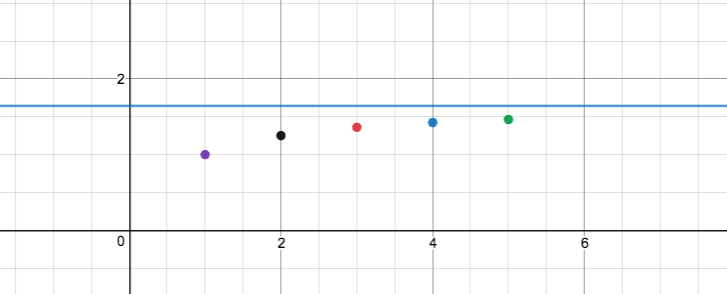
\includegraphics[height=4cm, width=8cm]{Images/graph.png}
\end{center}
The first point is the first partial sum and so on. We can see here that if we drew a line from point to point, it would form a graph that approaches the line of $\frac{\pi^2}{6}$. This just proves that $\frac{1}{k^2}$ converges to $\frac{\pi^2}{6}$.
\section*{Harmonic}
Let's look at the series of $\sum\limits_{k=1}^{\infty} \frac{1}{k}$. Let's start by listing out some terms in the series.
$$1+\frac{1}{2}+\frac{1}{3}...$$
This series diverges. Let's look at another similar series where we would group the terms together to see why this makes sense.
$$1+\frac{1}{2}+\frac{1}{2}+\frac{1}{4}+\frac{1}{4}+\frac{1}{8}+\frac{1}{8}+\frac{1}{8}+\frac{1}{8}...$$
We can see that as we group the quarters and the eighths together, we end up with 
$$1+\frac{1}{2}+\frac{1}{2}+\frac{1}{2}...$$
If we think about it, if we continue to add $\frac{1}{2}$ over and over again, it will eventually approach infinity. Since the terms of this series are less than the terms of the harmonic series, the terms must also add up to infinity. Let's look at another visual of partial sums.
$$S_1=1$$
$$S_2=1.5$$
$$S_3=1.8333$$
$$S_4=2.0833$$
$$S_5=2.2833$$
\begin{center}
    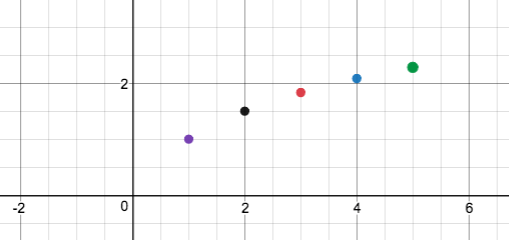
\includegraphics[height=4cm, width=7cm]{Images/graph2.png}
\end{center}
As we can see here, the points are growing larger and larger and diverges, just as we predicted.
\section*{One Over K Factorial}
Let's look at $\sum\limits_{k=0}^{\infty} \frac{1}{k!}$ Let's list out some terms.
$$\frac{1}{0!}+\frac{1}{1!}+\frac{1}{2!}+\frac{1}{3!}...$$
$$1+1+\frac{1}{2}+\frac{1}{6}...$$
This series converges to e, or about $2.71828$ Let's look at some partial sums to see if they end up approaching this number.
$$S_1=1$$
$$S_2=2$$
$$S_3=2.5$$
$$S_4=2.6667$$
We can see that the partial sums grow closer to $2.71828$ the more numbers we add together. Let's look at the partial sums on a graph.
\begin{center}
    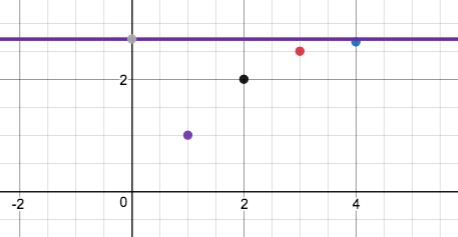
\includegraphics[height=4cm, width=7cm]{Images/graph3.png}
\end{center}
As we can see here, the partial sums are growing increasingly closer to e, which is graphed as a line. This confirms that it converges to e.
\section*{Collapsing}
Let's look at the collapsing series $\sum\limits_{k=1}^{\infty} \frac{1}{k(k+1)}$
Use partial sums to rewrite the expression.
$$\frac{1}{k(k+1)}=\frac{A}{k}+\frac{B}{k+1}$$
$$1=A(k+1)+Bk$$
Solve for A and B.
$$A=1|B=-1$$
This can be rewritten as $\sum\limits_{k=1}^{\infty} \frac{1}{k}-\frac{1}{k+1}$
Let's write some terms out. Since we're testing if the series converges or diverges as it approaches infinity, let's find the limit as it approaches infinity
$$\lim_{k\to\infty}(1-\frac{1}{2})+(\frac{1}{2}-\frac{1}{3})+(\frac{1}{3}...)+(-\frac{1}{k})+(\frac{1}{k}-\frac{1}{k+1})$$
If we cancel out all of the terms, we're left with
$$\lim_{k\to\infty}(1-\frac{1}{k+1})$$
As k approaches infinity, the denominator of the fraction grows larger and larger so it approaches 0. Therefore, we're just left with 1. Now, we know that the series converges to 1. Let's look at some partial sums and graph them to confirm that this is true.
$$S_1=0.5$$
$$S_2=0.6667$$
$$S_3=0.75$$
$$S_4=.8$$
Let’s look at these points on a graph now and see if it approaches 1.
\begin{center}
    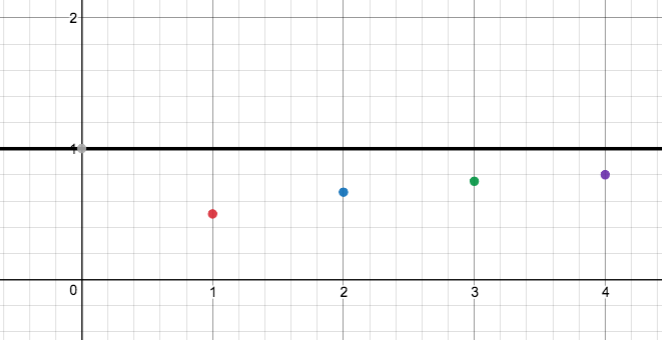
\includegraphics[height=4cm, width= 7cm]{Images/graph4.png}
\end{center}
As we can see here, the points are growing closer and closer to 1 as more terms are added to each other. This is just more proof that it converges to 1.
\section*{Alternating}
Let’s look at the alternating series $\sum\limits_{k=1}^{\infty}\frac{(-1)^{k+1}}{k}$
This series converges to ln(2), or 0.69314718056. Let‘s list out some terms to see the series‘ behavior.
$$1-\frac{1}{2}+\frac{1}{3}-\frac{1}{4}...$$
Now, let’s look at some partial sums.
$$S_1=1$$
$$S_2=0.5$$
$$S_3=0.8333$$
$$S_4=0.5833$$
$$S_5=0.7833$$
$$S_6=0.6167$$
Let’s look at these points on a graph and see if they approach 0.69314618056.
\begin{center}
    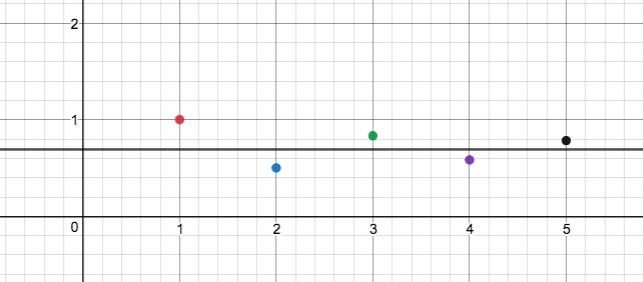
\includegraphics[height=4cm, width=7cm]{Images/graph5.png}
\end{center}
As we can see here, the points oscillate between being above and below 0.69314618056. The reason that they oscillate is because the sum switches from having positive and negative numbers being added. We can see them growing increasingly closer to the ln(2) the more numbers that are added to the sum, indicating that it converges to ln(2).
\end{document}
